\documentclass[english,11pt,a4paper]{article}
\usepackage[margin=1in]{geometry}
\usepackage{fontspec}
\setmainfont{lmroman10-regular.otf}[BoldFont=lmroman10-bold.otf,ItalicFont=lmroman10-italic.otf,BoldItalicFont=lmroman10-bolditalic.otf]
\setsansfont{lmsans10-regular.otf}[BoldFont=lmsans10-bold.otf]
\setmonofont{lmmono10-regular.otf}[Scale=MatchLowercase]
\newlength{\LeanCharWidth}
\usepackage{amsmath,amssymb}
\usepackage[english]{babel}
\usepackage{microtype,parskip}
\usepackage{graphicx,float,caption}
\usepackage{longtable,booktabs,array,calc}
\usepackage{xcolor}
\usepackage{xurl}
\usepackage{hyperref,bookmark}
\usepackage{etoolbox,needspace}
\setcounter{secnumdepth}{-\maxdimen}
\setlength{\emergencystretch}{3em}
\providecommand{\tightlist}{\setlength{\itemsep}{0pt}\setlength{\parskip}{0pt}}
\newcounter{none}
\AtBeginEnvironment{longtable}{\Needspace{8\baselineskip}\small}
\pretocmd{\section}{\Needspace{5\baselineskip}}{}{}
\pretocmd{\subsection}{\Needspace{4\baselineskip}}{}{}
\pretocmd{\subsubsection}{\Needspace{4\baselineskip}}{}{}
\captionsetup{font=small,labelfont=bf}
\urlstyle{same}
\clubpenalty=10000\widowpenalty=10000
\DeclareMathSizes{9}{10}{7}{5}
\hypersetup{pdflang={en-US},colorlinks=true,linkcolor=blue,urlcolor=blue,citecolor=blue}
\hypersetup{pdftitle={Stability of the Clique Partition Gap in Split Graphs},pdfauthor={Juan Pablo Traverso Gianini}}
\title{Stability of the Clique Partition Gap in Split Graphs}
\author{Juan Pablo Traverso Gianini\\\small Independent researcher, Santiago, Chile\\\small\href{mailto:jtraverso@gmail.com}{jtraverso@gmail.com}\quad\href{https://orcid.org/0009-0003-6068-4096}{ORCID 0009-0003-6068-4096}}
\date{Preprint 1.0 \enspace · \enspace November 23, 2026}
\begin{document}\raggedbottom\maketitle
\begin{center}\small Paper II in the series on clique partition gaps in split graphs.\end{center}
\noindent\textbf{DOI:} \url{https://doi.org/10.5281/zenodo.24452724}\\
\textbf{Official series repository:} \url{https://github.com/jtraverso/split-clique-partition-gap}\\
\textbf{Paper II repository:} \url{https://github.com/jtraverso/split-clique-partition-gap-ii}
\subsection{Abstract}\label{abstract}

In Part I {[}1{]}, we realized a residual packing gap by assigning core pairs to hosts. Here we study what can be deduced about the gap when some pairs lack an assignment. Let \(G\) be a split graph whose core is a clique of size \(c\), and suppose each host neighborhood is independent in the residual graph. If a proper assignment leaves \(L\) required pairs unassigned, the gap of \(G\) differs from the residual packing gap by at most \(2L\). One crossing-edge deletion attains the bound. The nearly quadratic gap of Part I survives arbitrary deletion of \(O(n^{2-\varepsilon})\) crossing edges for fixed \(\varepsilon>0\). Without changing the number \(n\) of vertices, we modify the padding hosts so that \(\Theta(n^2)\) crossing edges incident to them can be deleted with exactly the same gap, subject to a budget at each core vertex and with all originally assigned triangles intact. When only the neighborhoods are known, matching numbers of deficient lists control the loss. With \(2c\) hosts the gap is zero if each core vertex misses at most \(\lfloor c/2\rfloor\) of them, permitting \(c\lfloor c/2\rfloor\) missing crossing edges regardless of how the omitted sets overlap. We also recover pairs by independently choosing a matching at each host according to a fractional decomposition, or by choosing a single matching in the hypergraph of assignments.

\subsection{1. Partial host assignments}\label{partial-host-assignments}

The first paper in this series, \emph{Nearly Quadratic Additive Gaps for Edge-Clique Partitions of Split Graphs} {[}1{]}, constructed split graphs with a nearly quadratic gap. In this second paper we study the stability of the assignment that realizes that gap.

In a clique partition of a finite simple graph \(G\), each edge belongs to exactly one of the chosen cliques. Write \(\operatorname{cp}(G)\) for the least number of cliques in such a partition. A fractional clique partition assigns a nonnegative weight to each clique so that the weights on every edge sum to one, and the minimum total weight of such an assignment is \(\operatorname{cp}^{\ast}(G)\). Throughout, the cliques used as pieces have at least two vertices and may have arbitrary order. We write
\[
\Delta(G)=\operatorname{cp}(G)-\operatorname{cp}^{\ast}(G).
\]

Every integral partition is feasible for the fractional problem, so \(\Delta(G)\ge0\). Balogh, He, Krueger, Nguyen and Wigal {[}10, Theorem 1.10{]} prove that \(\Delta(G)=o(n^2)\) for graphs on \(n\) vertices. Their decomposition theorem gives this bound on taking \(t=2\) and assigning cost one to every clique.

The split graphs in the first paper {[}1{]} have a clique \(V\), called the core, and an independent set \(H\). A vertex \(h\in H\) is a \emph{host}, with neighborhood \(N_h\subseteq V\). In that construction, a graph \(B\) on \(V\) determines which core pairs require a host. Every such pair \(uv\) has a designated host \(h\) for which \(huv\) is a triangle. If the edge \(hu\) is deleted, the pair \(uv\) is still present in the core, but the designated triangle is gone. The question is how much of the original gap survives.

Chen, Erdős and Ordman {[}11{]} assign matchings in the core to vertices of the independent set to bound the integral partition number. When the crossing edges are all present, Chahua and Gutierrez {[}14, Lemma 2{]} use each assigned vertex to extend its matching to edge-disjoint triangles.

Fix a graph \(B\) on \(V\) and put \(J=\binom{V}{2}\setminus E(B)\). All pairs of \(V\) are edges of the split graph \(G\), including the pairs in \(J\). For \(Q\subseteq V\) with \(|Q|\ge2\), let \(e_B(Q)\) be the number of edges of \(B\) with both ends in \(Q\), and give \(Q\) the score
\[
w(Q)=2e_B(Q)-\binom{|Q|}{2}-1.
\]

Since every pair of \(Q\) lies in exactly one of \(E(B)\) and \(J\), the score can also be written as \[
w(Q)=\left(\binom{|Q|}{2}-1\right)-2\left|J\cap\binom{Q}{2}\right|.
\]

The first term counts the saving from covering all edges of \(Q\) with a single piece. The second deducts two for each required pair occupied by that piece. Each such pair could otherwise support a host triangle, replacing three individual edges with one piece.

A \emph{residual packing} is a collection of such sets in which each pair of \(V\) occurs at most once. Write \(I(B)\) for its maximum total score, allowing the empty collection. In a fractional residual packing, the variables \(y_Q\ge0\) satisfy
\[
\sum_{Q\supseteq e}y_Q\le1 \qquad \left(e\in\binom{V}{2}\right).
\]

Write \(F(B)\) for the maximum of \(\sum_Q y_Qw(Q)\). This maximum exists because every \(Q\) contains a pair, so \(y_Q\le1\), and the feasible set is a closed subset of a finite-dimensional unit cube. The empty packing is feasible in both problems.

A \emph{proper host assignment} on \(J_0\subseteq J\) chooses, for each \(uv\in J_0\), a host \(h\) with \(u,v\in N_h\). The pairs assigned to any one host must form a matching. The assigned triangles are pairwise edge-disjoint because their core edges are distinct and any two using the same host have disjoint core endpoints. We use host assignments in the sense of {[}3, §5{]}.

\textbf{Theorem 1 (stability of host transfer).} Suppose that each \(N_h\) is independent in \(B\). If \(J_0\subseteq J\) admits a proper host assignment and \(L=|J\setminus J_0|\), then
\[
\big|\Delta(G)-(F(B)-I(B))\big|\le 2L. \tag{1}
\]

When \(J_0=J\), (1) recovers the exact gap identity in {[}1, Lemma 2.1{]}. For an incomplete assignment, we adjoin a private host of degree two for each unassigned pair and then restrict the resulting graph to its original vertices. After applying Theorem 1 to crossing-edge deletions in Section 3, we turn to the assignments that can be recovered from the surviving neighborhoods. We use the list-coloring tools of Paper VI {[}4{]} to bound the loss through matchings on deficient lists in Section 4, then exploit overlapping choices through matching polytopes in Section 5 and pseudorandom hypergraph matchings in Section 6.

\subsection{2. The proof of stability}\label{the-proof-of-stability}

\textbf{Lemma 2 (exact transfer {[}1, Lemma 2.1{]}).} Under the hypotheses of Theorem 1, if \(J_0=J\), then
\[
\begin{aligned}
\operatorname{cp}(G)   &= |E(G)|-2|J|-I(B),\\
\operatorname{cp}^{\ast}(G) &= |E(G)|-2|J|-F(B).
\end{aligned} \tag{2}
\]

\emph{Proof.} Use the partition into individual edges as a reference. A clique \(K\) saves \(\binom{|K|}{2}-1\) pieces. The same count holds for fractional partitions. Indeed, if \(x_K\) denotes the weight of \(K\), summing the unit loads over the edges gives
\[
|E(G)|=\sum_{e\in E(G)}\sum_{K\supseteq e}x_K
       =\sum_K x_K\binom{|K|}{2}.
\]

The partition into single edges costs \(|E(G)|\). A fractional partition costs \(\sum_K x_K\), since one unit of weight costs one unit regardless of clique size. Its saving is the difference
\[
\begin{aligned}
\underbrace{|E(G)|-\sum_K x_K}_{\text{total saving}}
 &=\sum_K x_K\binom{|K|}{2}-\sum_K x_K\\
 &=\sum_K x_K\left(\binom{|K|}{2}-1\right).
\end{aligned}
\]

For an integral partition, \(x_K=1\) for each chosen clique and \(x_K=0\) otherwise, so the last sum adds the savings of the individual pieces.

Put \(j(Q)=|J\cap\binom{Q}{2}|\). Since \(e_B(Q)+j(Q)=\binom{|Q|}{2}\), the saving on a clique contained in the core is
\[
\binom{|Q|}{2}-1=w(Q)+2j(Q). \tag{3}
\]

A clique outside the core contains one host and \(u\ge1\) of its neighbors. It covers \(\binom u2\) core pairs and \(u\) crossing edges, at a cost of one piece. All its core pairs belong to \(J\) by neighborhood independence. To bound its saving, allow two units for each of those pairs. The unused allowance is
\[
2\binom u2-\left(\binom{u+1}{2}-1\right)
=\binom u2-u+1
=\frac{u(u-1)-2u+2}{2}
=\frac{(u-1)(u-2)}2.
\]

For \(u=1\) the piece is a single edge and saves zero. For \(u=2\) a triangle saves exactly the two units allowed by its one core pair. For \(u=3\) a four-vertex clique saves five pieces against an allowance of six. The factored expression is nonnegative for every integer \(u\ge1\). Now take any clique partition. Its core cliques form a residual packing, so their total score is at most \(I(B)\). The additional charges from (3) and from the cliques containing hosts sum to at most \(2|J|\), since each pair of \(J\) is covered once. With fractional weights, the core cliques satisfy the same pair capacities, and the total weight at each pair of \(J\) is still one. The saving is therefore at most \(I(B)+2|J|\) in the integral case and \(F(B)+2|J|\) in the fractional case.

For the reverse bounds, start with an optimal residual packing. Write \(y_Q\) for its coefficients, using zero and one in the integral case, and set \(\ell_e=\sum_{Q\supseteq e}y_Q\) for each core pair \(e\). Keep the core cliques at weights \(y_Q\). For each \(e=uv\in J\) with assigned host \(h\), give \(huv\) weight \(1-\ell_e\). This fills \(e\) to weight one. The matching condition ensures that the crossing edges \(hu\) and \(hv\) occur in no other assigned triangle, so their loads also remain at most one. Give each edge of \(G\) its remaining weight as an individual edge. This is an exact fractional partition. If the starting coefficients are integral, every remaining weight is zero or one, and the same construction is an integral partition.

By (3), the core cliques save \(\sum_Q y_Qw(Q)+2\sum_{e\in J}\ell_e\). The assigned triangles save \(2\sum_{e\in J}(1-\ell_e)\), and the individual edges contribute zero saving. Addition gives the residual score plus \(2|J|\) in each case. Subtracting these savings from \(|E(G)|\) proves (2).

\textbf{Lemma 3 (induced restriction).} Let \(K\) be an induced subgraph of a finite simple graph \(X\). Suppose that the graph with edge set \(E(X)\setminus E(K)\) admits a clique partition with \(p\) pieces. Then
\[
|\Delta(X)-\Delta(K)|\le p. \tag{4}
\]

\emph{Proof.} Intersect each clique of a partition of \(X\) with \(V(K)\) and discard intersections of size less than two. Every remaining set is a clique of \(K\). Each edge of \(K\) still belongs to the restriction of its unique original piece. Hence \(\operatorname{cp}(K)\le\operatorname{cp}(X)\).

For a fractional partition, add the weights of all cliques with the same surviving intersection. For any edge \(ab\) of \(K\), the cliques contributing at \(ab\) are precisely the original cliques containing \(a\) and \(b\). Their total weight remains one. Discarding the smaller intersections can only decrease the cost. Thus \(\operatorname{cp}^{\ast}(K)\le\operatorname{cp}^{\ast}(X)\) as well.

Conversely, adjoin the \(p\) given cliques to an optimal partition of \(K\). Their edges are disjoint from \(E(K)\) and cover all the remaining edges of \(X\). This increases the integral cost by \(p\), and assigning weight one to the same \(p\) cliques gives the corresponding fractional extension. The increments \(\operatorname{cp}(X)-\operatorname{cp}(K)\) and \(\operatorname{cp}^{\ast}(X)-\operatorname{cp}^{\ast}(K)\) both lie in \([0,p]\). Their difference lies in \([-p,p]\), which proves (4).

\emph{Proof of Theorem 1.} For each \(e=uv\in J\setminus J_0\), add a distinct vertex \(h_e\) with neighborhood \(\{u,v\}\). Call the resulting graph \(G^+\). Since \(uv\notin E(B)\), the new neighborhood is independent in \(B\). Assign \(e\) to \(h_e\) and retain the old assignment on \(J_0\). The pairs at an old host still form the same matching, and a new host receives only one pair. Formula (2) therefore gives \(\Delta(G^+)=F(B)-I(B)\).

The original vertices induce \(G\) in \(G^+\). The edges outside \(G\) are exactly \(h_eu,h_ev\) for the \(L\) new hosts. Taking these \(2L\) edges individually in Lemma 3 gives (1).

For an illustration with a three-vertex core, take \(V=\{u,v,w\}\), \(E(B)=\{uw\}\) and one host \(h\) with neighborhood \(\{u,v\}\). The assignment realizes \(uv\) but misses \(vw\). In Figure 1 the dotted edges are the two added in the proof. Deleting their common endpoint recovers the original graph, including the core edge \(vw\).

\begin{figure}[htbp]
\centering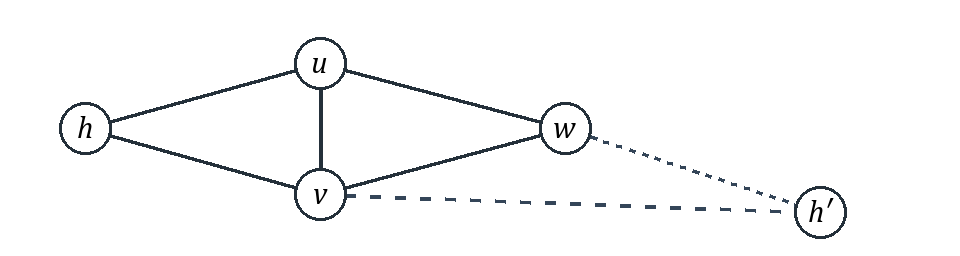
\includegraphics[width=.73\linewidth]{figures/private-host.png}
\caption{Completing the assignment at the pair $vw$. The solid edges, including the core edge $vw$, belong to the original split graph.}\label{fig:private-host}
\end{figure}

\textbf{Lemma 4 (unused capacity on missing pairs).} Under the hypotheses of Theorem 1, write \(M=J\setminus J_0\) and \(\Phi(B)=F(B)-I(B)\). Let \(\ell_e^I\) and \(\ell_e^F\) be the loads of any chosen optimal integral and fractional residual packings. Then \[
\Phi(B)-2\sum_{e\in M}(1-\ell_e^F)
\ \le\ \Delta(G)\ \le\
\Phi(B)+2\sum_{e\in M}(1-\ell_e^I). \tag{5}
\]

\emph{Proof.} Write \(A=|E(G)|-2|J|\). The upper bounds on savings in the first half of Lemma 2 used only the independence of the host neighborhoods. They give the two lower bounds \(A-I(B)\le\operatorname{cp}(G)\) and \(A-F(B)\le\operatorname{cp}^{\ast}(G)\). For the upper bounds on costs, carry out the construction in the second half using only the triangles assigned on \(J_0\). For any residual packing of score \(s\) and loads \(\ell_e\), its core cliques save \(s+2\sum_{e\in J}\ell_e\), and the available triangles save \(2\sum_{e\in J_0}(1-\ell_e)\). The remaining edge capacities are filled individually, so the resulting cost is \(A-s+2\sum_{e\in M}(1-\ell_e)\). Integral input again gives integral output. Let \(R_I\) and \(R_F\) denote twice the total unused capacity on \(M\) in the chosen integral and fractional optima. The bounds just proved give \[
\begin{aligned}
A-I(B)&\le\operatorname{cp}(G)\le A-I(B)+R_I,\\
A-F(B)&\le\operatorname{cp}^{\ast}(G)\le A-F(B)+R_F.
\end{aligned}
\] Subtracting the upper endpoint of the second interval from the lower endpoint of the first gives \(\Phi(B)-R_F\). The opposite endpoints give \(\Phi(B)+R_I\), proving (5).

In particular, equality \(\Delta(G)=\Phi(B)\) still holds if an integral optimum and a fractional optimum each saturate every missing pair. Proposition 5a attains the constant two with one crossing-edge deletion from a complete assignment.

\subsection{3. Deleting crossing edges from a witness}\label{deleting-crossing-edges-from-a-witness}

In their estimate for the integral partition number, Chen, Erdős and Ordman {[}11{]} count the designated triangles lost to missing crossing edges. Here the surviving triangles give a partial assignment. Theorem 1 then controls the change in the difference of the two partition numbers.

\textbf{Corollary 5.} Let \(G\) have a complete assignment as in (2). If \(G'\) is obtained from \(G\) by deleting \(q\) edges between \(V\) and \(H\), then
\[
|\Delta(G')-\Delta(G)|\le 2q. \tag{6}
\]

\emph{Proof.} A pair keeps its designated host if both crossing edges of its triangle survive. For each lost pair, one of the deleted edges witnesses the loss. These witness edges are distinct because two pairs incident to \(u\) and assigned to \(h\) would violate the matching condition at \(h\). Thus at most \(q\) pairs are lost, even when both crossing edges of a designated triangle are deleted.

The remaining pairs keep a proper assignment in \(G'\). Shrinking a host neighborhood preserves its independence in \(B\), and the core and \(B\) are unchanged. Apply Theorem 1 to \(G'\) and substitute \(F(B)-I(B)=\Delta(G)\) from (2).

For the witnesses of {[}1, Theorem 1.1{]}, there are absolute constants \(a_0>0\) and \(n_0\) such that for each \(n\ge n_0\) the original gap is at least
\[
f(n)=\frac{a_0 n^2}{(\log n)^{5/2}}
      \exp\!\left(-2\sqrt{\log(24/7)\log n}\right),
\]

where logarithms are natural. After any \(q_n\) crossing-edge deletions the resulting graph still has \(n\) vertices, including hosts left isolated, and (6) gives \(\Delta(G'_n)\ge f(n)-2q_n\). In particular, for fixed \(\varepsilon>0\) and \(q_n=O(n^{2-\varepsilon})\), the ratio \(q_n/f(n)\) tends to zero. Indeed its logarithm, when \(q_n>0\), is at most \[
-\varepsilon\log n+2\sqrt{\log(24/7)\log n}+\tfrac52\log\log n+O(1),
\] which tends to \(-\infty\). Thus \(\Delta(G'_n)\ge(1-o(1))f(n)\), whether or not the deletions preserve connectivity.

\textbf{A gap that rises and falls.} On the core \(V=\{0,1,2,3,4,5\}\) take \[
E(B)=\{05,12,14,15,23,24,25,34,45\},
\] where \(ij\) denotes the unordered pair \(\{i,j\}\). Each of the six remaining pairs has its own host adjacent to its two ends. First delete the edge from the host of \(01\) to \(0\), then the edge from the host of \(03\) to \(0\). Corollary 5 keeps \(B\) fixed to bound the change. To compute the optima exactly in each row, we instead move the affected pair into \(B\) after each deletion. The affected host now has degree one, so its neighborhood remains independent in the enlarged residual graph. The other hosts still realize a complete assignment on the new \(J\). In deletion order the pairs \((|E(G)|,|J|)\) are \((27,6),(26,5),(25,4)\), so the common term \(|E(G)|-2|J|\) in (2) takes the values \(15,16,17\).

\begin{center}
\begin{tabular}{cccccc}
\toprule
Crossing edges deleted & $I(B)$ & $F(B)$ & $\operatorname{cp}(G)$ & $\operatorname{cp}^{\ast}(G)$ & $\Delta(G)$ \\
\midrule
Neither & 5 & 5 & 10 & 10 & 0 \\
At $01$ & 5 & 6 & 11 & 10 & 1 \\
At $01$ and $03$ & 6 & 6 & 11 & 11 & 0 \\
\bottomrule
\end{tabular}
\end{center}

Writing a string of vertices for the corresponding subset of \(V\), fractional packings attaining the three values use, respectively, the set \(12345\) with weight one, the four sets \(0125,0145,1234,2345\) with weight one half each, and the whole core with weight one. For upper bounds, assign nonnegative prices to pairs so that the sum on every subset \(Q\) is at least \(w(Q)\). In the first row the nonzero prices are \(15:2,\ 24:3\). In the second they are \(15:3,\ 24:2,\ 34:1\). In the third they are two on \(15\), one on \(24\), and one half on each of \(12,14,23,25,34,45\). Summing the price inequalities against a feasible fractional packing counts each price at most once. The price totals are \(5,6,6\).

In the middle row, an integral packing of score six would attain the total dual price. It would therefore cover each positive-price pair \(15,24,34\) and use only tight sets, those whose score equals the sum of their pair prices. Checking the subsets containing \(34\) gives just two tight choices, \(1234\) and \(2345\). The tight choices containing \(15\) are \(0125,0145,1245,01245\). Each choice in the first list shares a pair with each choice in the second, so an integral packing cannot attain six. The sets \(234\) and \(0145\) share only vertex \(4\) and have scores two and three. They attain five.

For the integral optima let \(T(A)\) be the maximum residual score using only the available core pairs \(A\). If no positive-score subset has all its pairs in \(A\), then \(T(A)=0\). Otherwise \(T(A)\) is the maximum of zero and \(w(Q)+T(A\setminus\binom Q2)\) over those subsets. The recursion is exact because any nonempty optimal positive-score packing contains one such \(Q\) and its other pieces avoid every pair of \(Q\). The verification script in {[}8{]} evaluates \(T\) on the fifteen available pairs and checks every price and packing inequality in exact rational arithmetic. The respective maximizing packings include \(1245\), the pair of sets \(234,0145\), and \(012345\). Substitution in (2) gives the two partition numbers in each row.

These unit changes add over arbitrarily many copies. For a disjoint union of residual graphs, projecting a piece \(Q\) onto its \(m\) nonempty block intersections gives a total of the block scores exceeding \(w(Q)\) by the number of cross-block pairs in \(Q\) minus \((m-1)\). This difference is nonnegative since there are at least \(\binom m2\) such pairs. In this calculation a singleton has score \(-1\), so dropping it only increases the projected score. Projection preserves capacities within each block, and conversely block packings can be combined without conflict. This proves additivity of both residual optima, also for fractional coefficients. On the union core, supply private hosts for all cross-block pairs as well as the original hosts in each block. One deletion per copy then raises the gap by \(q\) on \(q\) copies. Starting at the middle row in each copy and making the second deletion lowers it by \(q\).

\textbf{Proposition 5a (sharpness).} The coefficient two in (6) is optimal. Equality also occurs in (1) with \(L=1\).

\emph{Proof.} On the eight core vertices \(0,\ldots,7\) take \[
J=\{14,15,17,35,36,46,47,56,57,67\}.
\] Set \(E(B)=\binom{V}{2}\setminus J\). Give each pair its own degree-two host. Delete the crossing edge joining vertex \(1\) to the host of \(14\). To evaluate (2) after deletion, move \(14\) into the residual. The nine surviving assignments are complete for the new required set, and the tenth host has a singleton neighborhood. The baseline in (2) goes from \(48-2(10)=28\) to \(47-2(9)=29\).

\begin{center}
\begin{tabular}{cccccc}
\toprule
State & $I$ & $F$ & $\operatorname{cp}$ & $\operatorname{cp}^{\ast}$ & $\Delta$ \\
\midrule
Before & $11$ & $35/3$ & $17$ & $49/3$ & $2/3$ \\
After & $11$ & $41/3$ & $18$ & $46/3$ & $8/3$ \\
\bottomrule
\end{tabular}
\end{center}

The integral packing \(245\), \(237\), \(034\), \(0126\) scores eleven in both states. The recurrence for \(T\) above, started with all 28 pairs, gives eleven as its upper bound in each case. For the fractional packing, use weight \(4/9\) on each of \(016\), \(037\), \(045\), \(126\), \(237\), \(245\), \(0134\), \(1234\), weight \(2/9\) on \(0256\), \(0257\), \(0267\), and weight \(1/9\) on \(134\), \(0126\), \(0237\), \(0245\). Before deletion the dual prices are \(1/3\) on \(05\), \(06\), \(07\), \(25\), \(26\), \(27\), \(2/3\) on \(16\), \(37\), \(45\), \(1\) on \(01\), \(03\), \(04\), \(12\), \(23\), \(24\), and \(5/3\) on \(02\), with zero elsewhere. Their sum is \(35/3\). Adding two to the price of \(14\) maintains dual feasibility in the second state because precisely the sets containing that pair gain two in score. The packing saturates \(14\) and attains both dual values. The verification script in {[}8{]} checks the 28 capacities and all 247 subset inequalities in each state and evaluates the integer recurrence.

Thus one deletion increases the gap by two. With the original residual held fixed, the same deletion leaves exactly one missing pair and gives \(\Delta(G')-\Phi(B)=2\). The disjoint-copy construction above gives an increase of \(2q\) for \(q\) deletions.

\textbf{Proposition 6 (changes to the residual graph).} Suppose \(B,B'\) are graphs on the same core and \(b=|E(B)\mathbin{\triangle} E(B')|\). Then \[
|\Phi(B')-\Phi(B)|\le 2b. \tag{7}
\] \emph{Proof.} Adding one edge \(e\) raises the score of any fixed feasible packing by twice its load at \(e\), an amount in \([0,2]\). The feasible sets depend only on the core pairs. Evaluating an optimal packing for \(B\) under the score function \(w_{B'}\) shows that neither optimum can decrease. Evaluating an optimal packing for \(B'\) under \(w_B\) bounds each increase by two. The difference between the two increases therefore lies in \([-2,2]\). Reversing the argument handles a deletion, and summing along the \(b\) edits gives (7). For split graphs with respective independent host neighborhoods and assignments missing \(L,L'\) pairs, (1) at both ends yields \(|\Delta(G')-\Delta(G)|\le 2(L+b+L')\).

\textbf{Proposition 6a (protected old assignments).} Let the residual on the old core \(U=U_0\sqcup U_1\sqcup U_2\) have these three independent classes and a complete assignment by old hosts. Adjoin \(W\) as isolated vertices of the residual, keeping all old assignments and all host neighborhoods independent in the enlarged residual. Write \(w=|W|\ge v=|U|\). For each class supply a separate family \(H_i\) of \(w+v+r\) new hosts with neighborhood \(W\cup U_i\), where \(r\ge0\) is an integer. Form \(G'\) from the resulting split graph \(G\) by deleting crossing edges. Suppose each core vertex loses at most \(b=\lfloor(v+r)/2\rfloor\) incidences in the union of the three families. If \(q_0\) deleted edges belong to the original assigned triangles on \(U\), then \[
|\Delta(G')-\Delta(G)|\le 2q_0.
\]

\emph{Proof.} For each pair in \(W\times U_i\) at least \(w+v+r-2b\ge w\) hosts in its family still see both ends. The maximum degree of this bipartite request graph is at most \(w\), so Galvin's list edge-coloring theorem {[}9{]} gives a proper assignment within each family. Families for different classes are disjoint. At each vertex of \(W\) this stage occupies at most \(v\) hosts, one for each old core neighbor. For an internal pair of \(W\), remove from its list the hosts unavailable at either end and those already used at either end. At least \[
3(w+v+r)-2b-2v\ge 3w+2r\ge w
\] hosts remain available for each internal pair of \(W\). Häggkvist--Janssen {[}2{]} now assigns all internal pairs, with disjoint crossing edges at each host. The old assigned triangles use other hosts. Each deleted edge there destroys at most one such triangle, leaving at most \(q_0\) missing pairs. Applying the same construction before deletion gives a complete assignment. Applying (2) before deletion and (1) after deletion compares both gaps with the same difference of residual optima.

For the witnesses of {[}1, §§5--6{]}, \(w=\lceil n/5\rceil\) and \(v=\Theta(n/\sqrt{\log n})\) as calculated in Section 6. With \(r=0\), deleting \(\lfloor v/2\rfloor\) incidences at each vertex of \(W\) in the three families already permits \(\Theta(n^2/\sqrt{\log n})\) deletions with unchanged gap. To obtain a quadratic budget at the same order, take \(r=\lfloor n/100\rfloor\). Before the final padding, the construction uses \(n_0+4w+3v\le24n/25+4\) vertices because \(v\le n_0\le n/25\). For sufficiently large \(n\), the remaining \(n/25-4\) vertices guaranteed by this count suffice to provide \(3r\) padding hosts. In each family, we connect \(r\) of these padding hosts to \(U_i\) in addition to \(W\). This preserves independence and the old assigned triangles. Adding isolated vertices to the residual preserves both packing optima {[}1, §5{]}, so the modified graph has the original gap. At each vertex of \(W\) one may now delete any \(b\) incidences to the three families. This gives \(wb=\Theta(n^2)\) deletions with \(q_0=0\) and hence exactly the original nearly quadratic gap.

\subsection{4. Reading the loss from the host lists}\label{reading-the-loss-from-the-host-lists}

Write \(c=|V|\) and regard \(J\) also as the graph of required pairs on \(V\). The list at \(e=uv\) is \(L_e=\{h\in H:u,v\in N_h\}\). Let \(k\) be a nonnegative integer such that every assignment of lists of size at least \(k\) to the edges of \(J\) admits a proper edge coloring from those lists. Equivalently, \(k\ge\chi'_\ell(J)\). For \(1\le t\le k\), define \[
d_k(e)=(k-|L_e|)_+,\qquad
E(D_t^{(k)})=\{e\in J:d_k(e)\ge t\},
\] where \(x_+=\max\{x,0\}\). Each deficiency graph has vertex set \(V\). We write \(\nu(D)\) for its maximum matching size.

\textbf{Proposition 7 (short lists).} If every \(N_h\) is independent in \(B\), then \[
|\Delta(G)-(F(B)-I(B))|\le 2\sum_{t=1}^{k}\nu(D_t^{(k)}). \tag{8}
\]

\emph{Proof.} The hosts serve as colors. Besides them we use distinct auxiliary colors \(\alpha_1,\ldots,\alpha_k\). Each \(e\in J\) receives the list \[
L_e\cup\{\alpha_t:1\le t\le d_k(e)\},
\] of size at least \(k\). In a proper coloring from these lists, the pairs receiving a host color form a proper host assignment. Every remaining pair has a unique auxiliary color \(\alpha_t\), whose entire color class is a matching in \(D_t^{(k)}\). Hence the sum in (8) counts an upper bound on the number of discarded pairs, even when a pair belongs to several deficiency levels. Theorem 1 gives the claim.

Häggkvist and Janssen {[}2, Theorem 1.1{]} show that lists of size \(c\) suffice for \(K_c\). They also suffice for \(J\), since arbitrary lists of that size on the other core pairs extend the instance to \(K_c\). If \(J\) has maximum degree \(d\ge1\), an edge meets at most \(2d-2\) other edges. Coloring in any order from lists of size \(2d-1\) therefore always leaves a color available. Either argument applies, giving \(k=\min\{c,2d-1\}\). For a nonempty matching one may take \(k=1\). For empty \(J\) the assignment is complete and Theorem 1 applies directly.

The graphs \(D_t^{(k)}\) are nested. With \(d_{\max}=\max_{e\in J}d_k(e)\) (zero for empty \(J\)), at most \(d_{\max}\) of them have edges, so the bound in (8) is at most \(2d_{\max}\nu(D_1^{(k)})\) for \(k\ge1\). Small vertex covers give convenient certificates for these matching numbers. For example, if all deficient pairs meet the same two vertices, each level contributes at most two. More generally, by the Tutte--Berge formula {[}13, Chapter 3{]} (formalized in {[}7{]}), any \(S\subseteq V\) certifies the upper bound \((c+|S|-o(D_t^{(k)}-S))/2\), where \(o\) counts odd components, and some \(S\) attains equality.

In the next corollary we take \(k=c\) and abbreviate \(D_t^{(c)}\) to \(D_t(J)\).

Okechukwu {[}12, Lemma 4.1{]} uses lists of common exterior neighbors to extend core edges to triangles. His proof reserves separate palettes and applies Galvin's theorem between two halves of the core. The following bound measures how the missing incidences are distributed among individual core vertices.

\textbf{Corollary 8.} For every split presentation with core \(V\), put \(J=\binom{V}{2}\) and form the graphs \(D_t(J)\) from the given neighborhoods. Then
\[
\Delta(G)\le 2\sum_{t=1}^{c}\nu(D_t(J)). \tag{9}
\]

If \(|H|\ge2c\), let \(M_u=\{h\in H:u\notin N_h\}\) and \(s_u=(|M_u|-\lfloor c/2\rfloor)_+\). Then \[
\Delta(G)\le 2\sum_{u\in V}s_u. \tag{10}
\] In particular, if at most \(r\) vertices have positive excess \(s_u\) and each excess is at most \(r\), then \(\Delta(G)\le2r^2\). This gives \(\Delta(G)\le2c\) whenever \(r^2\le c\).

\emph{Proof.} Take \(B\) to be the edgeless graph on \(V\). Every host neighborhood is independent in \(B\), and each residual set \(Q\) has score \(-\binom{|Q|}{2}-1<0\). The empty packing attains both optima at zero, giving (9) from (8) with \(k=c\).

For each pair \(uv\) we have \[
|L_{uv}|=|H|-|M_u\cup M_v|\ge 2c-2\lfloor c/2\rfloor-s_u-s_v\ge c-s_u-s_v .
\] Give each \(u\) its own set \(A_u\) of \(s_u\) auxiliary colors. These sets are mutually disjoint and avoid the hosts. The list \(L_{uv}\cup A_u\cup A_v\) has at least \(c\) colors, so {[}2{]} gives a proper coloring. A color belonging to \(A_u\) is available only on edges incident to \(u\), and properness allows at most one of those edges to use it. Discarding the edges with auxiliary colors therefore loses at most \(\sum_u s_u\) pairs. The remaining colors give a proper host assignment, and (1) yields (10). Under the stated hypothesis the sum has at most \(r\) nonzero terms of size at most \(r\).

For \(2c\) hosts, suppose each core vertex misses an arbitrary set of \(\lfloor c/2\rfloor\) of them. Then \(c\lfloor c/2\rfloor\) crossing edges are absent, yet every core pair has at least \(c\) common hosts. Every positive deficiency level is empty, so \(\Delta(G)=0\) (permitting \(5{,}000\) missing crossing edges when \(c=100\)). Conversely, a gap of size \(g\) forces the sum of the matching numbers in (9) to be at least \(g/2\) in every split presentation.

\subsection{5. Redundancy at individual hosts}\label{redundancy-at-individual-hosts}

A list records the choices for one pair. To keep track of choices that can be used together, consider the graph \(J_h\) of required pairs within \(N_h\). For each \(h\) let \(x^h\) be a nonnegative vector on its edges, extended by zero on other pairs. Suppose the sum of its entries incident to each vertex is at most one and \[
\sum_{e\in E(J_h[U])}x^h_e\le (|U|-1)/2
\] for every odd set \(U\subseteq N_h\). These are Edmonds' matching polytope inequalities {[}5{]}. Set \(\lambda_e=\sum_h x^h_e\) and \(p_e=\prod_h(1-x^h_e)\), using one for the empty product.

\textbf{Theorem 9 (recovery from overlapping choices).} If each \(N_h\) is independent in \(B\), then \[
|\Delta(G)-\Phi(B)|\le 2\sum_{e\in J}p_e
                  \le 2\sum_{e\in J}\exp(-\lambda_e). \tag{11}
\] More precisely, (5) holds with each of its two sums replaced by \(\sum_{e\in J}p_e(1-\ell_e)\), using the corresponding fractional or integral optimum.

\emph{Proof.} Edmonds' theorem expresses \(x^h\) as a convex combination of incidence vectors of matchings of \(J_h\). Drawing a matching with those probabilities selects \(e\) at \(h\) with probability \(x^h_e\). We draw independently at different hosts. A pair is missed with probability exactly \(p_e\), and \(p_e\le\exp(-\lambda_e)\) follows from \(1-x\le e^{-x}\) for \(x\ge0\). When a pair is selected at several hosts, we keep it at the first in a fixed order. Removing the other copies preserves the matching at each host, so each outcome gives a proper partial assignment. Inequality (5) holds on every outcome with the same \(\Delta(G)\) and the same chosen optimal packings. Taking expectations on its two sides gives the weighted bounds. Since \(0\le1-\ell_e\le1\), they imply (11).

For a family on \(n\) vertices with \(\Phi(B)\ge f(n)\) as in Section 3, a sufficient condition for preserving \((1-o(1))f(n)\) is \(\min_{e\in J}\lambda_e\ge(C+\gamma)\sqrt{\log n}\), where \(C=2\sqrt{\log(24/7)}\) and \(\gamma>0\) is fixed. Indeed \(|J|\le n^2\), and the ratio of the error in (11) to \(f(n)\) is at most \((2/a_0)(\log n)^{5/2}\exp(-\gamma\sqrt{\log n})\), which tends to zero. Here \(a_0\) is the leading constant in \(f(n)\) from Section 3.

The witnesses with universal vertices in {[}1, §§5--6{]} illustrate a limitation of this condition. They have a set \(W\) of \(w=\lceil n/5\rceil\) core vertices isolated in \(B\) and adjacent to every host. Fix \(u\in W\). All \(w-1\) pairs from \(u\) to \(W\setminus\{u\}\) have the full host list, yet the degree constraint at \(u\) gives \[
\sum_{v\in W\setminus\{u\}}\lambda_{uv}\le |H|.
\] Consequently some such pair has \(\lambda_{uv}\le |H|/(w-1)\le(n-w)/(w-1)=4+o(1)\). The uniform threshold of order \(\sqrt{\log n}\) therefore exceeds the redundancy available in this presentation, whose robustness in Section 3 follows from retaining the designated triangles.

\subsection{6. Simultaneous recovery}\label{simultaneous-recovery}

To record both causes of conflict between candidate triangles, form a hypergraph whose vertices are the required pairs and the crossing incidences \((h,u)\) with \(u\in N_h\), taken as disjoint classes. A candidate \(huv\) gives the hyperedge \(\{uv,(h,u),(h,v)\}\). A matching selects each pair at most once and uses each crossing edge at most once, precisely the conditions for a proper partial assignment. Two pair vertices never lie in one hyperedge. A pair and an incidence determine the host and both endpoints, and two incidences in one hyperedge also determine the triangle. Thus distinct vertices have codegree at most one.

\begin{figure}[htbp]
\centering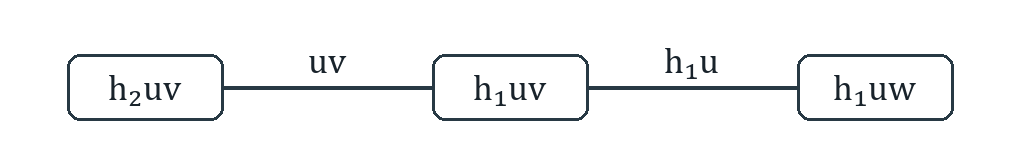
\includegraphics[width=.73\linewidth]{figures/triangle-conflicts.png}
\caption{The candidates $h_2uv$ and $h_1uv$ compete for the pair $uv$. The candidates $h_1uv$ and $h_1uw$ use the same crossing edge $h_1u$. The two outer candidates are compatible.}\label{fig:triangle-conflicts}
\end{figure}

Write \(S=\sum_{e\in J}|L_e|\) for the number of hyperedges. The degree of \(e\) is \(|L_e|\) and the degree of \((h,u)\) is \(d_{J_h}(u)\). Under neighborhood independence every pair of \(N_h\) belongs to \(J\), so the latter degree equals \(|N_h|-1\) for \(u\in N_h\). Both kinds of degrees enter the choice of \(D\) below.

\textbf{Proposition 10.} Fix \(0<\delta<1\) and put \(\epsilon=\delta/450\). For sufficiently large \(D\) depending on \(\delta\), suppose all the above degrees are at most \(D\) and \[
D^{1+\delta}\le S\le\exp(D^{\epsilon^2}).
\] Under the independence hypothesis of Theorem 1, \[
|\Delta(G)-\Phi(B)|\le
2\bigl(|J|-(1-D^{-\epsilon})S/D\bigr).
\]

\emph{Proof.} Apply the pseudorandom matching theorem of Ehard, Glock and Joos {[}6, Theorem 1.2{]} with uniformity three and the single edge weight function identically one. The codegree bound is at most \(D^{1-\delta}\), the number of hyperedges obeys the upper size bound, and the total weight \(S\) meets the lower bound for the theorem. There is a matching of size at least \((1-D^{-\epsilon})S/D\). Each of its hyperedges recovers one distinct pair, so Theorem 1 applies with at most \(|J|-(1-D^{-\epsilon})S/D\) missing pairs. If every list has size at least \((1-\eta)D\), with \(0\le\eta\le1\), substitution of \(S\ge(1-\eta)D|J|\) bounds the error by \(2(\eta+D^{-\epsilon})|J|\).

The degree formulas also give a test on the padded examples of {[}1{]}. Let \(n_0\le n/25\) be the order before enlargement, \(v_0\le n_0\) the original core size and \(w=\lceil n/5\rceil\). Take \(D=|H|\). This bounds every pair degree, and for sufficiently large \(n\) every incidence degree is at most \(v_0+w-1<|H|\). Pairs within \(W\) have degree \(|H|=n-v_0-w\). For \(u\in W\) and an original core vertex \(a\), the list of \(ua\) contains the old hosts that see \(a\) and exactly the \(v_0+w\) new color-class hosts for the class of \(a\). The final padding hosts see only \(W\). Thus \(|L_{ua}|\le n_0+v_0+w\), and \[
\frac{|L_{ua}|}{D}\le\frac{2n/25+w}{n-n/25-w}
      \le\frac7{19}+o(1).
\] In particular, the special case with \(\eta=o(1)\) does not apply to all pairs in these witnesses. We can also evaluate the order of the unweighted estimate. In the notation of {[}1, §6{]}, \(v_0=15m^{2j}\), \(j\) is of order \(\sqrt{\log n}\), and \(m\) is the largest odd integer at most \(X=(n/(25b_j))^{1/(2j)}\), where \(b_j=255+2880j\). Since \(X/j\to\infty\) and \(m>X-2\), we have \((m/X)^{2j}\to1\), giving \(v_0=\Theta(n/\sqrt{\log n})\). Now \(S\ge\binom w2D=\Theta(n^3)\) and \(S\le n^3\), so both size hypotheses hold eventually for every fixed \(\delta\in(0,1)\).

The normalized deficit is the sum of the unused proportions of the individual lists: \[
|J|-S/D=\sum_{e\in J}\bigl(1-|L_e|/D\bigr).
\] Every pair within \(W\) contributes zero. There are at most \(wv_0+\binom{v_0}{2}\) other pairs, while the \(wv_0\) pairs between \(W\) and the old core each contribute at least \(12/19-o(1)\). Thus \(|J|-S/D=\Theta(n^2/\sqrt{\log n})\). The additional term \(D^{-\epsilon}S/D\) is \(O(n^{2-\epsilon})\). On these unchanged witnesses the unweighted theorem therefore recovers a \(1-o(1)\) fraction of the required pairs, but its error bound is larger than \(f(n)\). Corollary 5 gives the stronger perturbation conclusion here.

\subsection{7. Formalization}\label{formalization}

The Lean 4 sources in {[}8{]} establish the two-sided transfer estimate (1), its refinement by the loads of the chosen optima (5), and both perturbation bounds (6) and (7). They also give the complete-core threshold \(k=c\) in (8), the endpoint excess bound (10), and the independent-matching estimate in (11) given finite matching decompositions. Compactness of the finite-dimensional feasible polytope identifies the supremum used in Lean with the maximum used here. The repository lists the declarations and their axioms, gives build instructions, and includes the exact verifiers for both examples in Section 3. The proof of Proposition 6a, the general list threshold, the replication argument and the asymptotic applications are given in the preceding sections.

The bilingual proof ledger accompanying {[}8{]} gives the calculation behind each result, including the equality case and the two stages of the padding construction.

\subsection{Acknowledgments}\label{acknowledgments}

The author is deeply grateful to his wife María Paz and his children Lucas, Juan Cristóbal, Francisca, Raimundo and Benjamín for their love, patience and support.

\subsection{Use of artificial intelligence and computational tools}\label{use-of-artificial-intelligence-and-computational-tools}

Claude, by Anthropic, and ChatGPT/Codex, by OpenAI, were used to explore and check arguments and to prepare the manuscript.

The author remains responsible for the arguments, citations, code and presentation. No AI system is listed as an author.

\subsection{References}\label{references}

{[}1{]} J. P. Traverso Gianini, \emph{Nearly Quadratic Additive Gaps for Edge-Clique Partitions of Split Graphs}, preprint 1.0 (2026), Theorem 1.1 and Lemma 2.1. \url{https://doi.org/10.5281/zenodo.24408988} · \url{https://github.com/jtraverso/split-clique-partition-gap}

{[}2{]} R. Häggkvist and J. Janssen, \emph{New bounds on the list-chromatic index of the complete graph and other simple graphs}, Combinatorics, Probability and Computing \textbf{6} (1997), 295--313, Theorem 1.1. \url{https://doi.org/10.1017/S0963548397002927}

{[}3{]} J. P. Traverso Gianini, \emph{Colorability and Realizability Defects in Resource-Dominated Packing Relaxations}, Paper V in the Erdős 81 series, §5. \url{https://github.com/jtraverso/erdos81-colorability-realizability-defects}

{[}4{]} J. P. Traverso Gianini, \emph{Optimal Clique Partitions under Local Perturbations}, Paper VI in the Erdős 81 series, Lean formalization. \url{https://github.com/jtraverso/erdos81-optimal-clique-partitions}

{[}5{]} J. Edmonds, \emph{Maximum Matching and a Polyhedron with 0,1-Vertices}, Journal of Research of the National Bureau of Standards B \textbf{69B} (1965), 125--130. \url{https://doi.org/10.6028/jres.069B.013}

{[}6{]} S. Ehard, S. Glock and F. Joos, \emph{Pseudorandom hypergraph matchings}, Combinatorics, Probability and Computing \textbf{29} (2020), 868--885, Theorem 1.2. \url{https://doi.org/10.1017/S0963548320000280}

{[}7{]} J. P. Traverso Gianini, \emph{Berge's augmenting path theorem and the Tutte--Berge formula}, Lean formalization. \url{https://github.com/jtraverso/berge-matching}

{[}8{]} J. P. Traverso Gianini, \emph{Split Gap II}, source code, build instructions and exact finite examples. \url{https://github.com/jtraverso/split-clique-partition-gap-ii}

{[}9{]} F. Galvin, \emph{The List Chromatic Index of a Bipartite Multigraph}, Journal of Combinatorial Theory, Series B \textbf{63} (1995), 153--158. \url{https://doi.org/10.1006/jctb.1995.1011}

{[}10{]} J. Balogh, J. He, R. A. Krueger, T. Nguyen and M. C. Wigal, \emph{Clique covers and decompositions of cliques of graphs}, Advances in Combinatorics \textbf{2026} (2026), Paper No.~9, Theorem 1.10. \url{https://doi.org/10.19086/aic/2026.9}

{[}11{]} G.-T. Chen, P. Erdős and E. T. Ordman, \emph{Clique partitions of split graphs}, in \emph{Combinatorics, Graph Theory, Algorithms and Applications} (Beijing, 1993), World Scientific, 1994, 21--30. \url{https://ordman.net/MathResearch/CEOClique_Parts.pdf}

{[}12{]} O. Okechukwu, \emph{Clique partitions and bounded simplicial defect}, arXiv:2609.20871 (2026), Lemma 4.1. \url{https://arxiv.org/abs/2609.20871}

{[}13{]} L. Lovász and M. D. Plummer, \emph{Matching Theory}, AMS Chelsea Publishing, 2009, Chapter 3. \url{https://doi.org/10.1090/chel/367}

{[}14{]} L. Chahua and J. Gutierrez, \emph{On Tuza's conjecture in dense graphs}, arXiv:2405.11409 (2024), Lemma 2. \url{https://arxiv.org/abs/2405.11409}

\end{document}
